\documentclass[10pt]{beamer}

%STANDARD PREAMBLE
%https://tex.stackexchange.com/questions/68821/is-it-possible-to-create-a-latex-preamble-header
\usepackage{/Users/miw267/Repos/latex_preamble/beamer_preamble}

% DOCUMENT SPECIFIC STUFF
% using default arg uments; see https://stackoverflow.com/questions/1812214/latex-optional-arguments




%%%% Citations should be rendered differently in beamer -- ADD TO BEAMER

\title{Lebesgue Integration}

\begin{document}

\maketitle

\section{Preface}

\begin{frame}{Goal}
In this section, we will introduce the general theory of integration of a function with respect to a general measure, as introduced by Lebesgue.  This is referred to as \textit{integration}, \textit{abstract integration}, or \textit{Lesbesgue integration}.

% We use use \textit{(Lesbesgue) integration against Lesbesgue measure} to refer to the special case of integrating a function defined on a sub-domain of the real line with respect to the Lebesgue measure. 
\end{frame}

\section{Integration}

\begin{frame}{Intuition}
Folland summarizes the difference between the Riemann and Lebesgue approaches thus: ``to compute the Riemann integral of $f$, one partitions the domain [...] into subintervals", while in the Lebesgue integral, ``one is in effect partitioning the range of $f$ " \cite{folland1999real}.

\end{frame} 
	
\begin{frame}{Intuition}

The figure below compares how the Riemann and Lesbesgue approaches would approximate the area under the curve of a function $f : \R \to \R$. 

\begin{figure}[H]
\centering 
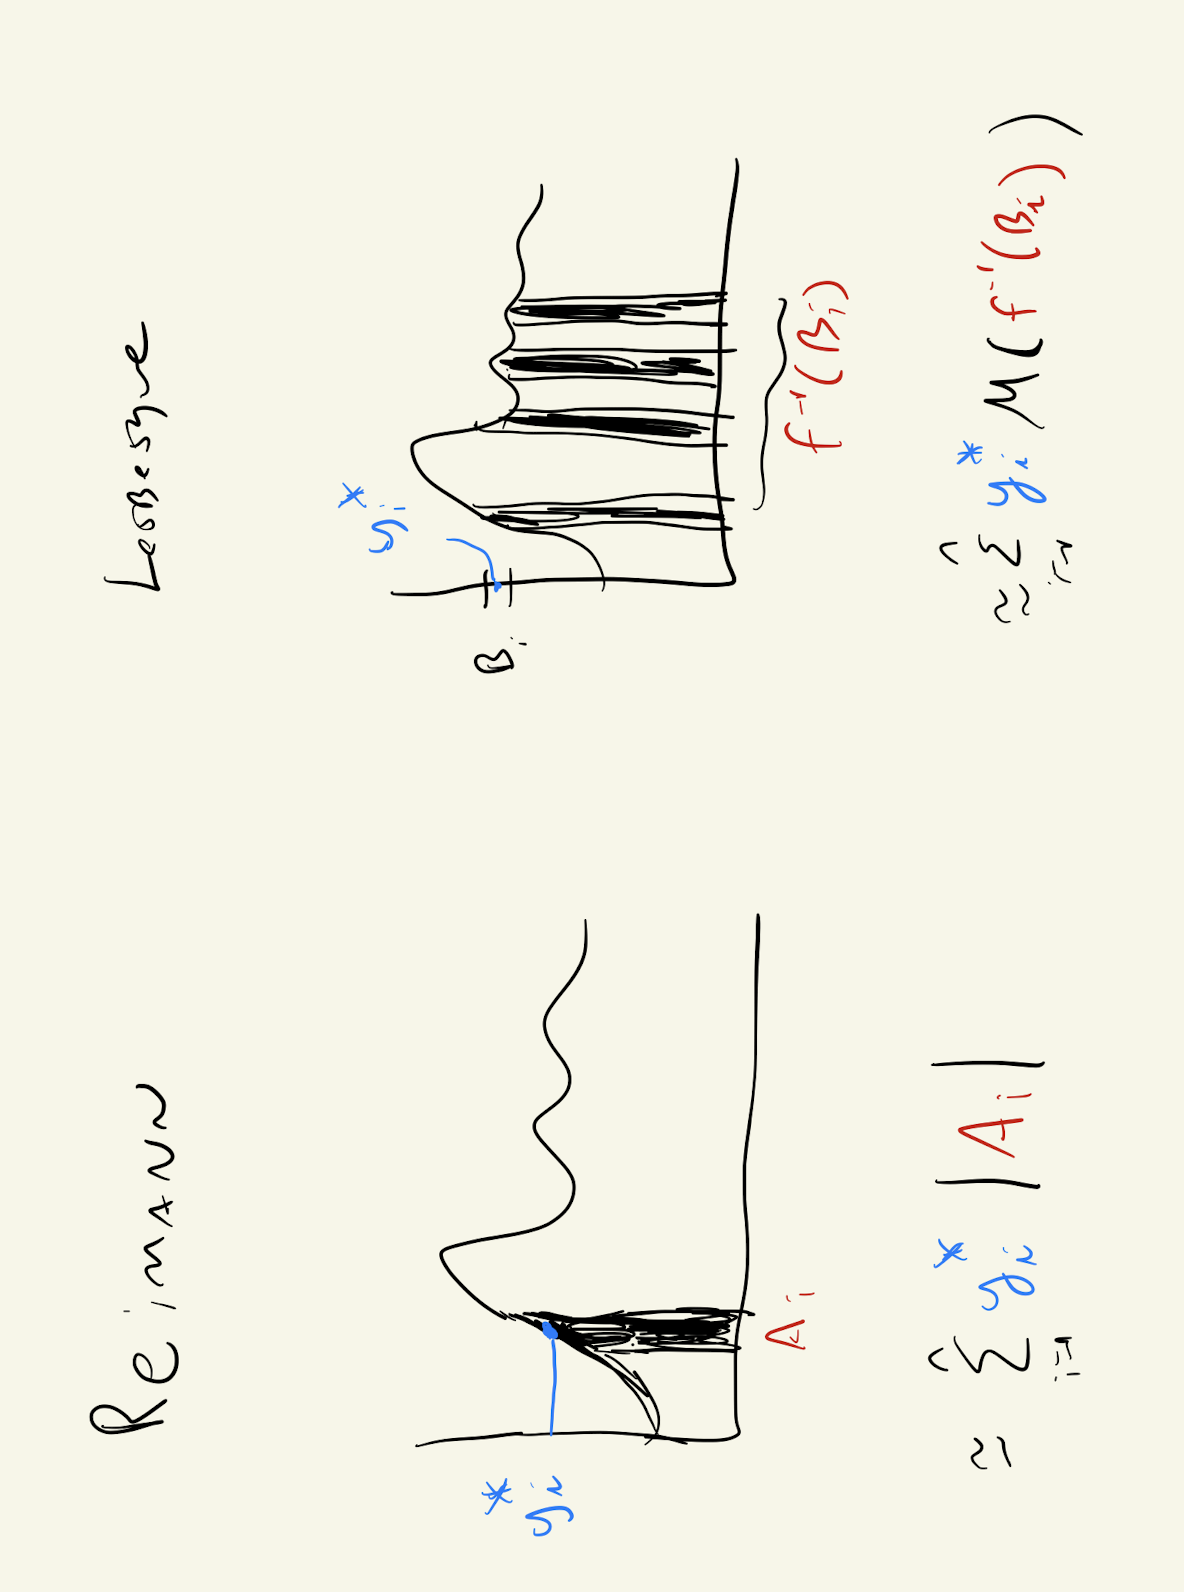
\includegraphics[width=.6\textwidth, angle=270]{images/lesbesgue_vs_reimann}
%\caption{Illustrating the fundamental differences between Reimann and Lesbesgue integration}
%\label{fig:lesbesgue_vs_reimann}
\end{figure}
\end{frame}



\begin{frame}[standout]{}
What differences do you see?
\end{frame}

\begin{frame}{One Difference -- Grouping values adaptively}

Since Lebesgue partitions the range and not the domain, it can \textit{group values adaptively} when computing the area under the curve as the sum over $n$ contributions.  

%Whereas a function can vary a lot in Reimann subintervals of the form $A_i = (a_i,b_i)$, in the Lesbesgue approach, the function will have controlled amount of variation for each of the $n$ contributions.  

The Lebesgue definition makes it possible to calculate integrals for a broader class of functions. 

For example, consider the \textit{Dirichlet function}, which is 0 where its argument is irrational and 1 otherwise.  The Reimann integral is undefined, because the upper sum and lower sum don't converge as the partition gets finer.

\end{frame}

\begin{frame}{One Difference -- Grouping values adaptively}
	

Lebesgue summarized his approach to integration in a letter to Paul Montel:
\begin{quotation}
I have to pay a certain sum, which I have collected in my pocket.  I take the bills and coins out of my pocket and give them to the creditor in the order I find them until I have reached the total sum. This is the Riemann integral. But I can proceed differently. After I have taken all the money out of my pocket I order the bills and coins according to identical values and then I pay the several heaps one after the other to the creditor. This is my integral.
\end{quotation}



The insight is that one should be able to rearrange the values of a function freely, while preserving the value of the integral.  This process of rearrangement can convert a very pathological function into one that is ``nice" from the point of view of integration %, and thus let such pathological functions be integrated.
\end{frame}

\begin{frame}{A second difference - Liberation from intervals}

We can integrate over arbitrary regions, that aren't necessarily intervals.

Consider: 
 
\[  \int_{x \, : \, \text{some condition on x holds}} f  \]

\end{frame}

\begin{frame}{A third difference - arbitrary measure}
	
The Reimann approach implicitly assumes that sets in the domain have sizes that are given by Lesbesgue measure ($\mu(A) = |A|)$, whereas the Lesbesgue approach allows sets in the domain to have sizes given by any arbitrary measure $\mu$.
\end{frame}

% Commented out because I don't think this is true.
%
%\begin{frame}{Yet another difference - more generalized domains}
%
%The Reimann approach assumes that the domain is totally ordered.  In contrast, Lesbesgue integrals can be defined for functions on arbitrary spaces.
%\end{frame}


\begin{frame}{Two-dimensional example}
Suppose we want to find a mountain's volume (above sea level).

\begin{itemize}
\item \textbf{The Riemann approach}: Divide the base of the mountain into a grid of 1 meter squares. Measure the altitude of the mountain at the center of each square. 
\item \textbf{The Lebesgue approach}: Draw a contour map of the mountain, where adjacent contours are 1 meter of altitude apart. 

\begin{figure}[H]
\centering 
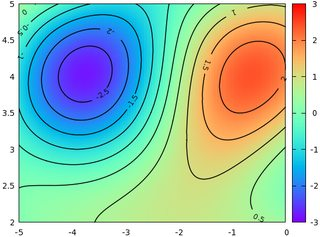
\includegraphics[width=.4\textwidth]{images/contour_plot}
\end{figure}
\end{itemize}
\end{frame}

%While the Riemann integral considers the area under a curve as made out of vertical rectangles, the Lebesgue definition considers slabs that are not necessarily just rectangles, and so it is more flexible. 

\begin{frame}[standout]
\begin{figure}[H]
\centering 
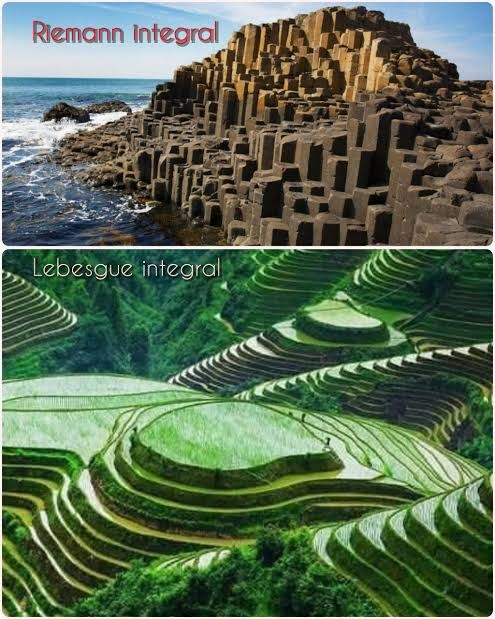
\includegraphics[width=.6\textwidth]{images/riemann_vs_lebesgue.jpg}
\end{figure}
\end{frame}



\begin{frame}{Notation}

Let $(\Omega, \F)$ be a measurable space, fixed throughout the discussion.

In this section, we define integral of a measurable function $h$ on $(\Omega, \F)$ against arbitrary measure $\mu$.  The integral can be written as:
\[ \ds\int_{\Omega} h \wrt{\mu}, \quad \quad \ds\int_{\Omega} h(\omega) \wrt{\mu(\omega)}, \quad \text{ or } \quad \ds\int_{\Omega} h(\omega) \mu(d \, \omega) \]
\vfill
{\tiny $h$ is measurable if the inverse image of every measurable set is measurable.}
\end{frame}
 
 

\begin{frame}{Integrals of simple functions}

\begin{definition}
Let $h$ be simple, say $h = \sum_{i=1}^r y_i I_{A_i}$ where the $A_i$ are disjoint sets in $\F$.  Then
\begin{align*}
\ds\int_{\Omega} h \wrt{\mu} := \ds\sum_{i=1}^r y_i \; \mu(A_i).
\labelit \label{eqn:integral_of_simple_function}	
\end{align*}
 \label{def:integral_of_simple_function}
\end{definition}

\begin{figure}[H]
\centering 
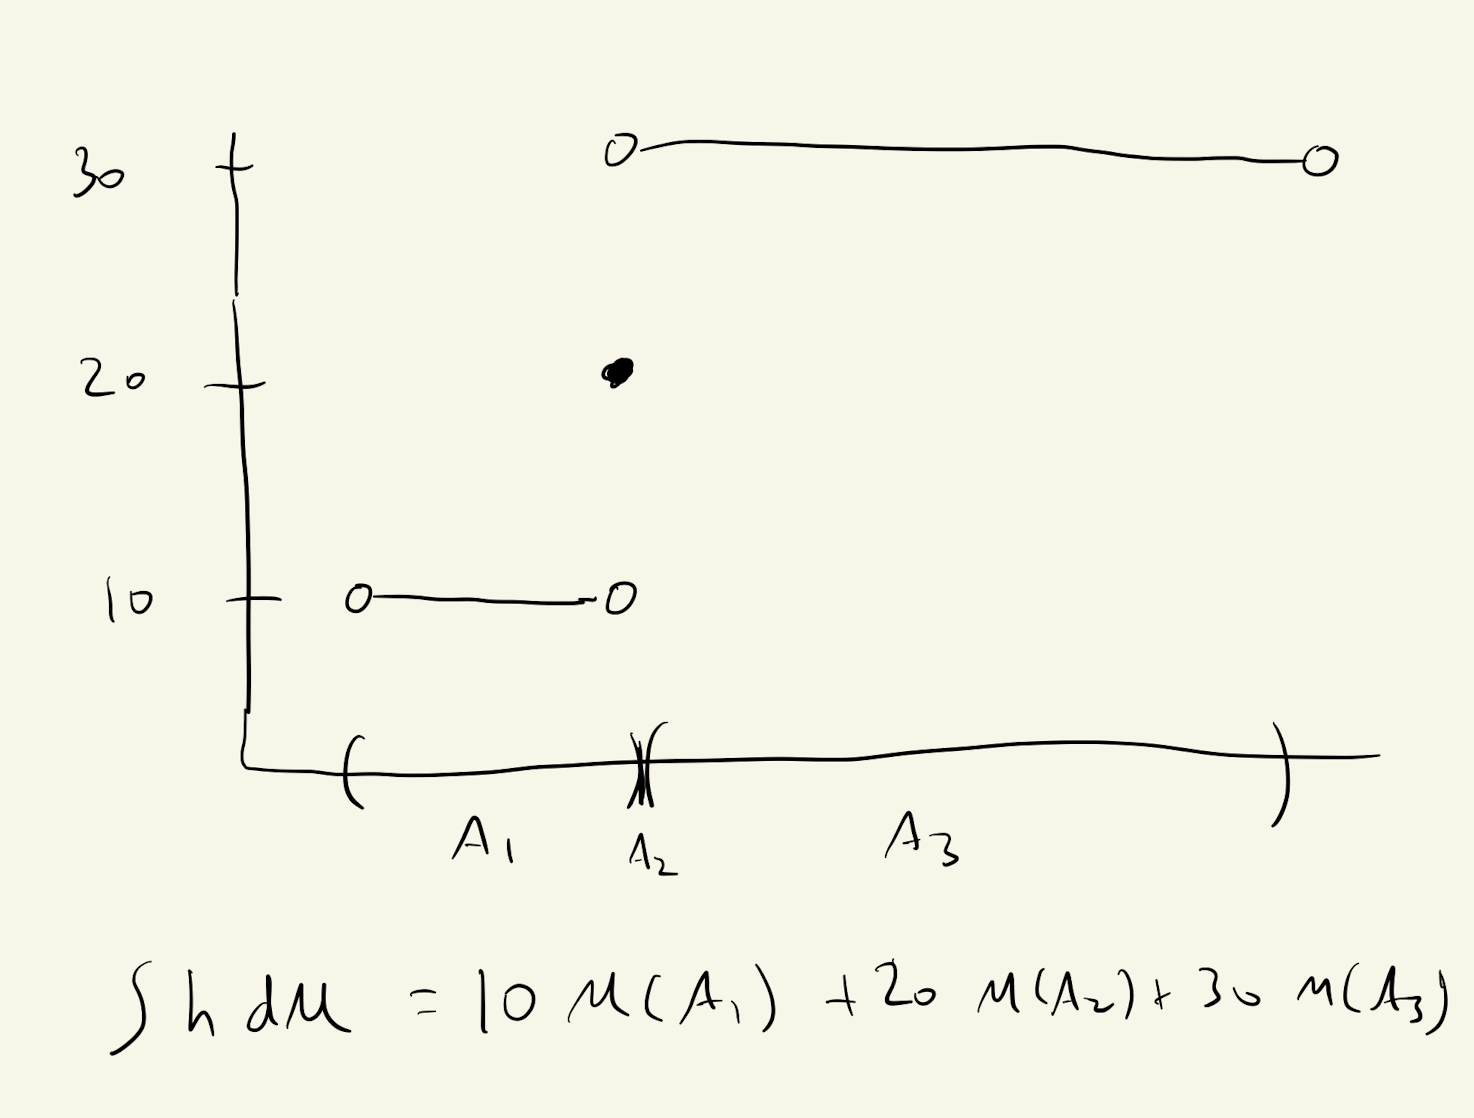
\includegraphics[width=.4\textwidth]{images/integral_of_simple_function}	
%\caption{The Lesbesgue integral of a simple function. {\scriptsize (In this case, the simple function is also a step function.)}}
\end{figure}	

{\tiny Note: The integral of a simple function exists whenever $\infty$ and  $-\infty$ do not both appear in the sum. } \\
{\tiny Example: Integrating the Dirichlet function (see notes).} 
\end{frame}

\begin{frame}{Integrals of non-negative Borel measurable functions}
\begin{definition}

If $h$ is non-negative Borel measurable, we define 

\[  \ds\int_{\Omega} h \wrt{\mu} = \sup \bigg\{ \ds\int_{\Omega} s \wrt{\mu} : s \quad \text{simple,} \quad 0 \leq s \leq h  \bigg\} \]
\label{def:integral_of_non_negative_Borel_measurable_function}
\end{definition}


\begin{figure}[H]
\centering
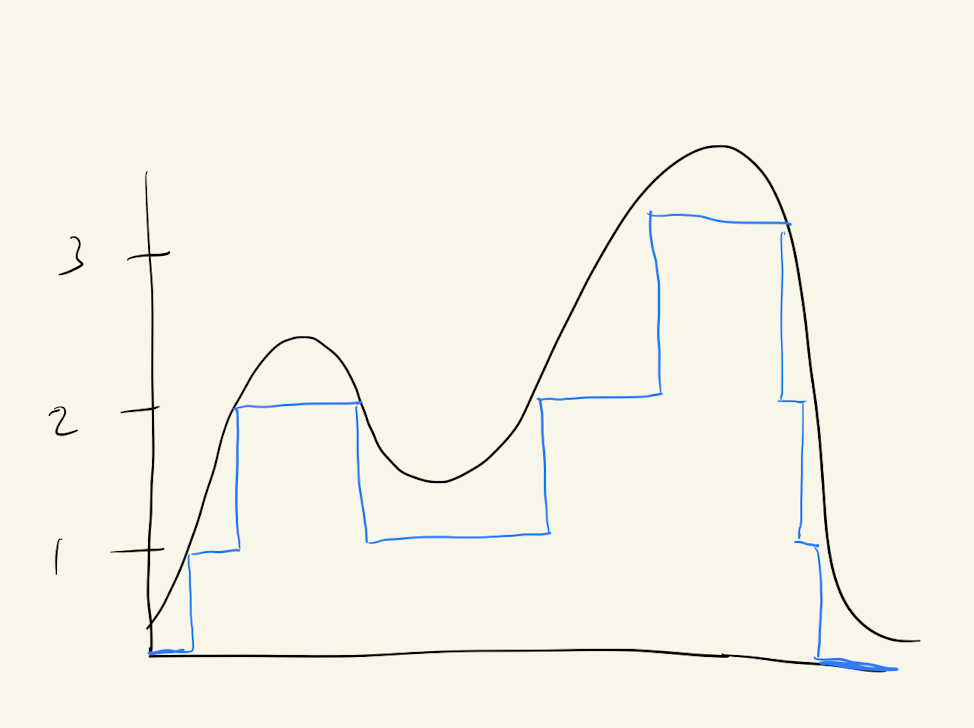
\includegraphics[width=.4\textwidth]{images/simple_function_approximating_non_negative_function}	
%\caption{A simple function approximating a non-negative function in terms of its integral}
\end{figure}

\bottomtext{The integral of a non-negative Borel measurable function \textit{always} exists (although it may take on the value $+\infty$).}
\end{frame}

\begin{frame}{Integrals of arbitrary Borel measurable functions}

Let $h$ be an arbitrary Borel measurable function.   We will express an arbitrary Borel measurable function as as the difference of two non-negative Borel measurable functions.


\begin{figure}[H]
\centering
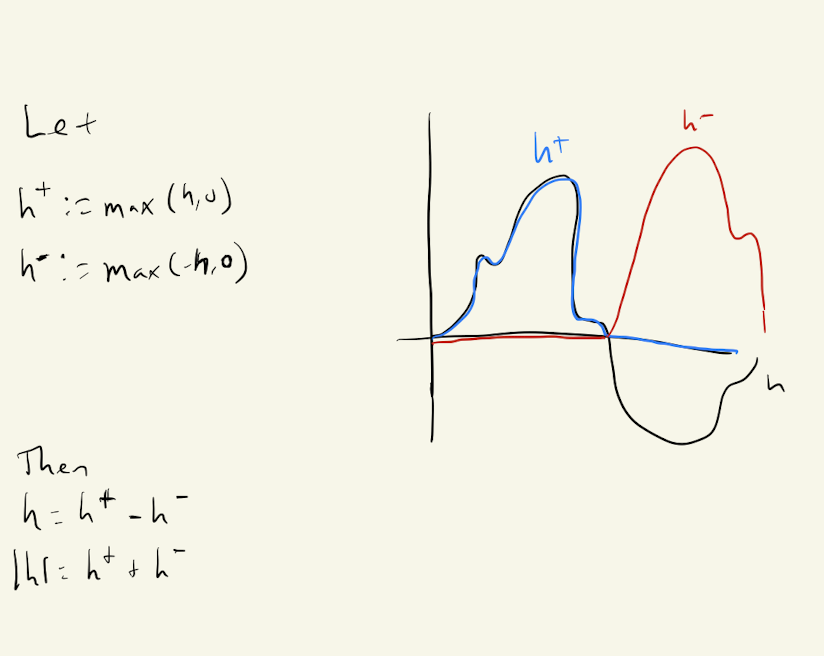
\includegraphics[width=.4\textwidth]{images/arbitrary_borel_measurable_functions_in_terms_of_nonnegative_borel_measurable_functions}
\end{figure}

We can define the integral of $h$ by 

\[ \ds\int_\Omega h \wrt{\mu} = \ds\int_\Omega h^+ \wrt{\mu} - \ds\int_\Omega h^- \wrt{\mu} \]

\vfill

\bottomtext{The integral of an arbitrary non-negative Borel function exists so long as it does not take the form $+\infty - \infty$.} 

\end{frame}

%\begin{frame}
%\begin{figure}[H]
%\centering 
%
\includegraphics[width=1.0\textwidth]{images/measure_theory_meme}
%\end{figure}
%\end{frame}

\end{document}



